\begin{frame}[label=title]
    \centering
    \begin{figure}[H]
        \includegraphics[keepaspectratio, width=0.7\paperwidth, height=.6\paperheight]{Logos/FreeFlower.pdf}
    \end{figure}
    Informatik: Data Science und Sicherheit\\
    \emoji{clamp}\textbf{Kompression}: Huffman-Kompression
\end{frame}

\begin{frame}{Huffman-Kodierung}
	\textbf{Idee}: Immer zuerst die Knoten mit den kleinsten Prozentzahlen verbinden
\end{frame}

\begin{frame}{Huffman-Kodierung: Algorithmus}
	\begin{itemize}[<+->]
		\small
		\item Jeder Buchstabe wird als Graph mit einem Knoten (=Baum mit einem Blatt) betrachtet. Die Häufigkeit jedes Buchstabens wird neben dem Blatt notiert. Wir wollen nun die Buchstaben zu Teilbäumen verbinden, bis wir einen einzigen Baum haben.
		\begin{figure}[H]
			\footnotesize
			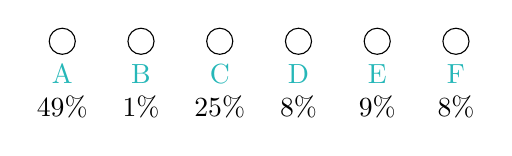
\begin{tikzpicture}
				\tikzstyle{n} = [text width=1cm,align=center, draw, shape=circle]
				\node[circle,draw, label={[align=center]below:\textcolor{BlueGreen}{A}\\ 49\%}, ](a){};
				\node[circle,draw, label={[align=center]below:\textcolor{BlueGreen}{B}\\ 1\%}, right of=a](b){};
				\node[circle,draw, label={[align=center]below:\textcolor{BlueGreen}{C}\\ 25\%}, right of=b](c){};
				\node[circle,draw, label={[align=center]below:\textcolor{BlueGreen}{D}\\ 8\%}, right of=c](d){};
				\node[circle,draw, label={[align=center]below:\textcolor{BlueGreen}{E}\\ 9\%}, right of=d](e){};
				\node[circle,draw, label={[align=center]below:\textcolor{BlueGreen}{F}\\ 8\%}, right of=e](f){};
			\end{tikzpicture}
			\normalsize
		\end{figure}
		\item In einer Schleife: Wir schauen alle isolierten Blätter und Wurzeln von Teilbäumen an. Die beiden Knoten mit den kleinsten Prozentzahlen werden miteinander verbunden. Die neue Wurzel wird markiert mit dem Prozentsatz beider Knoten.
		\begin{figure}[H]
			\footnotesize
			\begin{tikzpicture}[-,>=stealth',
				level distance=12mm,
				level 1/.style={sibling distance=15mm},
				level 2/.style={sibling distance=30mm},
				level 3/.style={sibling distance=15mm},
				level 4/.style={sibling distance=15mm},
				level 5/.style={sibling distance=15mm},
				leaf/.style={circle, draw},
				edge from parent path={(\tikzparentnode.south) -- (\tikzchildnode)}]


				\usetikzlibrary{shapes}
				\tikzstyle{n} = [align=center]
				\tikzstyle{r} = [text=red]

				\node[n]{\textcolor{BlueGreen}{B,D}\\ 9\%}[edge from parent]
				child {node[n] {\textcolor{BlueGreen}{B}\\ 1\%}
					edge from parent node[left,r]{};
				}
				child {node[n]{\textcolor{BlueGreen}{D}\\ 8\%}
					edge from parent node[r,right]{};
				};
			\end{tikzpicture}
			\normalsize
		\end{figure}
		\item Bei Gleichstand ist jede Wahl erlaubt (gleiche Gesamtlänge). Konvention: Teilbaum mit der geringsten Tiefe nehmen.
		\end{itemize}
		\only<4>{\textbf{Welche Knoten werden als nächstes miteinander verbunden?}}
\end{frame}

\begin{frame}{Huffman-Kodierung: Beispiel}
	\begin{figure}[H]
		\footnotesize
		\begin{tikzpicture}[-,>=stealth',
			level distance=15mm,
			level 1/.style={sibling distance=15mm},
			level 2/.style={sibling distance=30mm},
			level 3/.style={sibling distance=15mm},
			level 4/.style={sibling distance=15mm},
			level 5/.style={sibling distance=15mm},
			leaf/.style={circle, draw},
			edge from parent path={(\tikzparentnode.south) -- (\tikzchildnode)}]


			\usetikzlibrary{shapes}
			\tikzstyle{n} = [align=center]
			\tikzstyle{r} = [text=red]

			\node(bd)[n]{\textcolor{BlueGreen}{B,D}\\ 9\%}[edge from parent]
			child {node(b)[n] {\textcolor{BlueGreen}{B}\\ 1\%}
				edge from parent node[left,r]{} ;
			}
			child {node[n]{\textcolor{BlueGreen}{D}\\ 8\%}
				edge from parent node[r,right]{};
			};
			\node(ef)[n, left of=bd,xshift=-15mm]{\textcolor{BlueGreen}{E,F}\\ 17\%}[edge from parent]
			child {node(f)[n] {\textcolor{BlueGreen}{F}\\ 8\%}
				edge from parent node[left,r]{} ;
			}
			child {node[n]{\textcolor{BlueGreen}{E}\\ 9\%}
				edge from parent node[r,right]{};
			};
			\node[n, left of=f](c){\textcolor{BlueGreen}{C}\\ 25\%};
			\node[n, left of=c](a){\textcolor{BlueGreen}{A}\\ 49\%};
		\end{tikzpicture}
		\normalsize
	\end{figure}
	\centering
	$\rightarrow$ Weshalb haben wir einen Baum \{\textcolor{BlueGreen}{E,F}\} statt \{\textcolor{BlueGreen}{F,B,D}\} gemacht?
\end{frame}


\begin{frame}{Huffman-Kodierung: Beispiel}
	\begin{figure}[H]
		\footnotesize
		\begin{tikzpicture}[-,>=stealth',
			level distance=15mm,
			level 1/.style={sibling distance=30mm},
			level 2/.style={sibling distance=15mm},
			level 3/.style={sibling distance=15mm},
			level 4/.style={sibling distance=15mm},
			level 5/.style={sibling distance=15mm},
			leaf/.style={circle, draw},
			edge from parent path={(\tikzparentnode.south) -- (\tikzchildnode)}]

			\usetikzlibrary{shapes}
			\tikzstyle{n} = [align=center]
			\tikzstyle{r} = [text=red]

			\node(febd)[n]{\textcolor{BlueGreen}{F,E,B,D}\\ 26\%}[edge from parent]
				child{node(ef)[n]{\textcolor{BlueGreen}{E,F}\\ 17\%}
					child {node(f)[n] {\textcolor{BlueGreen}{F}\\ 8\%}
						edge from parent node[left,r]{} ;
					}
					child {node[n]{\textcolor{BlueGreen}{E}\\ 9\%}
						edge from parent node[r,right]{};
					}
					edge from parent node[r,right]{};
				}
				child{node(bd)[n]{\textcolor{BlueGreen}{B,D}\\ 9\%}
					child {node(b)[n] {\textcolor{BlueGreen}{B}\\ 1\%}
						edge from parent node[left,r]{} ;
					}
					child {node[n]{\textcolor{BlueGreen}{D}\\ 8\%}
						edge from parent node[r,right]{};
					}
					edge from parent node[r,left]{};
				};
			\node[n, left of=f](c){\textcolor{BlueGreen}{C}\\ 25\%};
			\node[n, left of=c](a){\textcolor{BlueGreen}{A}\\ 49\%};
		\end{tikzpicture}
		\normalsize
	\end{figure}
\end{frame}

\begin{frame}{Huffman-Kodierung: Beispiel}
	\begin{figure}[H]
		\footnotesize
		\begin{tikzpicture}[-,>=stealth',
			level distance=15mm,
			level 1/.style={sibling distance=60mm},
			level 2/.style={sibling distance=30mm},
			level 3/.style={sibling distance=30mm},
			level 4/.style={sibling distance=15mm},
			level 5/.style={sibling distance=15mm},
			leaf/.style={circle, draw},
			edge from parent path={(\tikzparentnode.south) -- (\tikzchildnode)}]

			\usetikzlibrary{shapes}
			\tikzstyle{n} = [align=center]
			\tikzstyle{r} = [text=red]

			\node(acebd)[n]{\textcolor{BlueGreen}{A,C,F,E,B,D}\\ 100\%}[edge from parent]
			child{node(a)[n]{\textcolor{BlueGreen}{A}\\ 49\%}
				edge from parent node[left,r]{} ;
			}
			child{node(cfebd)[n]{\textcolor{BlueGreen}{C,F,E,B,D}\\ 51\%}
				child{node(c)[n]{\textcolor{BlueGreen}{C}\\ 25\%}
					edge from parent node[left,r]{} ;
					}
				child{node(febd)[n]{\textcolor{BlueGreen}{F,E,B,D}\\ 26\%}
					child{node(ef)[n]{\textcolor{BlueGreen}{E,F}\\ 17\%}
						child {node(f)[n] {\textcolor{BlueGreen}{F}\\ 8\%}
							edge from parent node[left,r]{} ;
						}
						child {node[n]{\textcolor{BlueGreen}{E}\\ 9\%}
							edge from parent node[r,right]{};
						}
						edge from parent node[r,right]{};
					}
					child{node(bd)[n]{\textcolor{BlueGreen}{B,D}\\ 9\%}
						child {node(b)[n] {\textcolor{BlueGreen}{B}\\ 1\%}
							edge from parent node[left,r]{} ;
						}
						child {node[n]{\textcolor{BlueGreen}{D}\\ 8\%}
							edge from parent node[r,right]{};
						}
						edge from parent node[r,left]{};
					}
				edge from parent node[right,r]{};
				}
				edge from parent node[right,r]{};
			};
		\end{tikzpicture}
		\normalsize
	\end{figure}
	\centering
	$\rightarrow$ Welcher Binärcode hat \textcolor{BlueGreen}{B}? Welcher hat \textcolor{BlueGreen}{E}?
\end{frame}

\begin{frame}{Huffman-Kodierung: Beispiel}
	\begin{figure}[H]
		\footnotesize
		\begin{tikzpicture}[-,>=stealth',
			level distance=15mm,
			level 1/.style={sibling distance=60mm},
			level 2/.style={sibling distance=30mm},
			level 3/.style={sibling distance=30mm},
			level 4/.style={sibling distance=15mm},
			level 5/.style={sibling distance=15mm},
			leaf/.style={circle, draw},
			edge from parent path={(\tikzparentnode.south) -- (\tikzchildnode)}]

			\usetikzlibrary{shapes}
			\tikzstyle{n} = [align=center]
			\tikzstyle{r} = [text=red]

			\node(acebd)[n]{\textcolor{BlueGreen}{A,C,F,E,B,D}\\ 100\%}[edge from parent]
			child{node(a)[n]{\textcolor{BlueGreen}{A}\\ 49\%\\\textcolor{red}{0}}
				edge from parent node[left,r]{0} ;
			}
			child{node(cfebd)[n]{\textcolor{BlueGreen}{C,F,E,B,D}\\ 51\%}
				child{node(c)[n]{\textcolor{BlueGreen}{C}\\ 25\%\\\textcolor{red}{10}}
					edge from parent node[left,r]{0} ;
				}
				child{node(febd)[n]{\textcolor{BlueGreen}{F,E,B,D}\\ 26\%}
					child{node(ef)[n]{\textcolor{BlueGreen}{E,F}\\ 17\%}
						child {node(f)[n] {\textcolor{BlueGreen}{F}\\ 8\%\\\textcolor{red}{1100}}
							edge from parent node[left,r]{0} ;
						}
						child {node[n]{\textcolor{BlueGreen}{E}\\ 9\%\\\textcolor{red}{1101}}
							edge from parent node[r,right]{1};
						}
						edge from parent node[r,left]{0};
					}
					child{node(bd)[n]{\textcolor{BlueGreen}{B,D}\\ 9\%}
						child {node(b)[n] {\textcolor{BlueGreen}{B}\\ 1\%\\\textcolor{red}{1110}}
							edge from parent node[left,r]{0} ;
						}
						child {node[n]{\textcolor{BlueGreen}{D}\\ 8\%\\\textcolor{red}{1111}}
							edge from parent node[r,right]{1};
						}
						edge from parent node[r,right]{1};
					}
					edge from parent node[right,r]{1};
				}
				edge from parent node[right,r]{1};
			};
		\end{tikzpicture}
		\normalsize
	\end{figure}
	\centering
\end{frame}

\begin{frame}{Mittlere Codelänge}
	\textbf{Mittlere Codelänge} (Bit pro Zeichen) $=$ Summe von (relative Häufigkeit $\times$ Länge des Codeworts)
	\begin{itemize}
		\item Huffman: $0.49\times1 + 0.25\times2 + (0.08+0.09+0.01+0.08)\times4 = 2.03$
		\item Maximale Balance: $(0.49+0.01+0.25)\times2 + 0.09\times3 + (0.08+0.08)\times4 = 2.41$
		\item Feste Länge (6 Buchstaben): 3
	\end{itemize}
	Text mit 1000 Zeichen: Huffman ca. 2030 Bits, maximale Balance ca. 2410 Bits, feste Länge 3000 Bits
\end{frame}

\begin{frame}{Fazit}
	\begin{itemize}
		\item Strategie der \textbf{maximalen Balance}: \textit{top-down}-Ansatz (von Wurzel zu Blättern), kann zu suboptimalen Kodierungen führen
		\item \textbf{Huffman-Kodierung}: \textit{bottom-up}-Ansatz (von Blättern zur Wurzel), garantiert die kürzestmögliche Gesamtlänge des kodierten Texts (unter allen präfixfreien Kodierungen einzelner Buchstaben)
	\end{itemize}
\end{frame}

\begin{frame}[label=auftrag]{Auftrag}
	\begin{itemize}
		\item \aufgabebox{Aufgaben 1.11--1.14}
	\end{itemize}
\end{frame}

\begin{frame}{So arbeitet ZIP: DEFLATE}
	\begin{itemize}
		\item ZIP, gzip und PNG verwenden das Verfahren \textbf{DEFLATE}: zwei Stufen
	\end{itemize}
	\begin{figure}[H]
		\centering
		\small
		\begin{tikzpicture}[node distance=.6cm,
				stufe/.style={draw, rounded corners, minimum height=.8cm, font=\bfseries},
				daten/.style={align=center}]
			\node[daten] (text) {Text};
			\node[stufe, right=of text] (lz) {LZ77};
			\node[daten, right=of lz] (paare) {Zeichen\\und Paare};
			\node[stufe, right=of paare] (huff) {Huffman};
			\node[daten, right=of huff] (bits) {Bits};
			\draw[->] (text) -- (lz);
			\draw[->] (lz) -- (paare);
			\draw[->] (paare) -- (huff);
			\draw[->] (huff) -- (bits);
		\end{tikzpicture}
	\end{figure}
	\begin{itemize}
		\item LZ77 ersetzt Wiederholungen durch Paare (Abstand, Länge): Ganze Zeichenfolgen kehren wieder
		\item Huffman kodiert die übrigen Zeichen und die Zahlen der Paare: Einzelne Zeichen sind unterschiedlich häufig
	\end{itemize}
\end{frame}

\begin{frame}[t]{Beispiel: \texttt{HALLO HALLO HALLO}} % [t]: Overlays beginnen oben, kein Springen
	\footnotesize
	\only<1>{
		\begin{itemize}
			\item 17 Zeichen, Häufigkeiten L~6, H~3, A~3, O~3, \textvisiblespace~2
			\item 8 Bits pro Zeichen: $17 \cdot 8 = 136$ Bits
			\item Feste Codelänge: 5 Zeichen $\rightarrow$ 3 Bits, $17 \cdot 3 = 51$ Bits
			\item Maximale Balance: \{L,H\} gegen \{A,O,\textvisiblespace\} ergibt L~\texttt{00}, H~\texttt{01}, A~\texttt{10}, O~\texttt{110}, \textvisiblespace~\texttt{111}, also 39 Bits (andere Wahl bei Gleichstand: 40 Bits)
		\end{itemize}
	}
	\only<2>{
		\textbf{Nur Huffman}: $3\cdot2 + 3\cdot2 + 6\cdot2 + 2\cdot3 + 3\cdot3 = 39$ Bits
		\begin{figure}[H]
			\centering
			\begin{tikzpicture}[-,>=stealth',
					level distance=11mm,
					level 1/.style={sibling distance=50mm},
					level 2/.style={sibling distance=26mm},
					level 3/.style={sibling distance=16mm},
					edge from parent path={(\tikzparentnode.south) -- (\tikzchildnode)}]
				\tikzstyle{n} = [align=center]
				\tikzstyle{r} = [text=red]
				\node[n]{\textcolor{BlueGreen}{A,O,\textvisiblespace,H,L}\\ 17}
				child {node[n] {\textcolor{BlueGreen}{A,O}\\ 6}
					child {node[n] {\textcolor{BlueGreen}{A}\\ 3\\\textcolor{red}{00}}
						edge from parent node[left,r]{0}}
					child {node[n] {\textcolor{BlueGreen}{O}\\ 3\\\textcolor{red}{01}}
						edge from parent node[right,r]{1}}
					edge from parent node[left,r]{0}}
				child {node[n] {\textcolor{BlueGreen}{\textvisiblespace,H,L}\\ 11}
					child {node[n] {\textcolor{BlueGreen}{\textvisiblespace,H}\\ 5}
						child {node[n] {\textcolor{BlueGreen}{\textvisiblespace}\\ 2\\\textcolor{red}{100}}
							edge from parent node[left,r]{0}}
						child {node[n] {\textcolor{BlueGreen}{H}\\ 3\\\textcolor{red}{101}}
							edge from parent node[right,r]{1}}
						edge from parent node[left,r]{0}}
					child {node[n] {\textcolor{BlueGreen}{L}\\ 6\\\textcolor{red}{11}}
						edge from parent node[right,r]{1}}
					edge from parent node[right,r]{1}};
			\end{tikzpicture}
		\end{figure}
	}
	\only<3>{
		\textbf{DEFLATE, Stufe 1 (LZ77)}: \texttt{H A L L O \textvisiblespace{} (6,11)}, Paar als Baustein \texttt{P}\\
		\textbf{Stufe 2 (Huffman)}: 18 Bits für die Codewörter, dazu Abstand und Länge mit je 5 Bits, also 28 Bits
		\begin{figure}[H]
			\centering
			\begin{tikzpicture}[-,>=stealth',
					level distance=11mm,
					level 1/.style={sibling distance=50mm},
					level 2/.style={sibling distance=26mm},
					level 3/.style={sibling distance=16mm},
					edge from parent path={(\tikzparentnode.south) -- (\tikzchildnode)}]
				\tikzstyle{n} = [align=center]
				\tikzstyle{r} = [text=red]
				\node[n]{\textcolor{BlueGreen}{P,L,H,A,O,\textvisiblespace}\\ 7}
				child {node[n] {\textcolor{BlueGreen}{P,L}\\ 3}
					child {node[n] {\textcolor{BlueGreen}{P}\\ 1\\\textcolor{red}{00}}
						edge from parent node[left,r]{0}}
					child {node[n] {\textcolor{BlueGreen}{L}\\ 2\\\textcolor{red}{01}}
						edge from parent node[right,r]{1}}
					edge from parent node[left,r]{0}}
				child {node[n] {\textcolor{BlueGreen}{H,A,O,\textvisiblespace}\\ 4}
					child {node[n] {\textcolor{BlueGreen}{H,A}\\ 2}
						child {node[n] {\textcolor{BlueGreen}{H}\\ 1\\\textcolor{red}{100}}
							edge from parent node[left,r]{0}}
						child {node[n] {\textcolor{BlueGreen}{A}\\ 1\\\textcolor{red}{101}}
							edge from parent node[right,r]{1}}
						edge from parent node[left,r]{0}}
					child {node[n] {\textcolor{BlueGreen}{O,\textvisiblespace}\\ 2}
						child {node[n] {\textcolor{BlueGreen}{O}\\ 1\\\textcolor{red}{110}}
							edge from parent node[left,r]{0}}
						child {node[n] {\textcolor{BlueGreen}{\textvisiblespace}\\ 1\\\textcolor{red}{111}}
							edge from parent node[right,r]{1}}
						edge from parent node[right,r]{1}}
					edge from parent node[right,r]{1}};
			\end{tikzpicture}
		\end{figure}
	}
	\only<4>{
		\begin{table}[H]
			\centering
			\begin{tabular}{lrr}
				\textbf{Verfahren} & \textbf{Bits} & \textbf{Ersparnis} \\\midrule
				(8 Bits pro Zeichen) & (136) & \\
				Feste Codelänge (3 Bits) & 51 & 0\% \\
				Maximale Balance & 39 & 23.5\% \\
				Huffman & 39 & 23.5\% \\
				DEFLATE (LZ77 und Huffman) & 28 & 45.1\%
			\end{tabular}
		\end{table}
		\centering
		Ersparnis gegenüber fester Codelänge $= 1 - \text{Bits}/51$
	}
\end{frame}

\begin{frame}{ZIP als Container}
	\begin{itemize}
		\item Eine ZIP-Datei enthält eine oder mehrere Dateien
		\item Pro Datei: Name, Datum, komprimierte Daten (DEFLATE) und eine Prüfsumme (CRC-32)
		\item Beim Entpacken erkennt das Programm mit der Prüfsumme, ob die Daten beschädigt sind (Thema Datenintegrität)
	\end{itemize}
\end{frame}

\begin{frame}{Auftrag}
	\begin{itemize}
		\item \aufgabebox{Aufgaben 1.15, 1.16}
	\end{itemize}
\end{frame}
